\subsection{Securing Multiple Processes in Multiple Enclaves}
\label{sec:gsgx:multiproc}

Upon existing platforms using \sgx{}, there is no
multi-process abstractions of any kinds that has been supported so far.
%either in \haven{} or other systems.
The main challenge for multi-process support in enclaves
is that enclaves cannot share pages,
to support either Linux-style copy-on-write forking or
sharing abstraction states across processes.
\graphene{} implements multi-process support
in zero-sharing fashion.
The multi-process abstraction supported by \graphene{} thus also \graphenesgx{}
includes {\tt fork}, {\tt execve}, signals, System V IPC, etc.
%The {\it zero-sharing} nature of \graphene{} makes it possible
%to support multi-process abstractions in enclaves
%without any architecture changes.

In this section we will describe how \graphenesgx{} securely creates
processes in new enclaves,
for supporting {\tt fork} and {\tt execve},
and implements inter-process communication
(namespace coordination, signals, System V IPC, etc)
with process isolation.

%\subsection{Forking into New Enclave}
%\label{sec:gsgx:multiproc:fork}

\begin{figure}[t!]
\centering
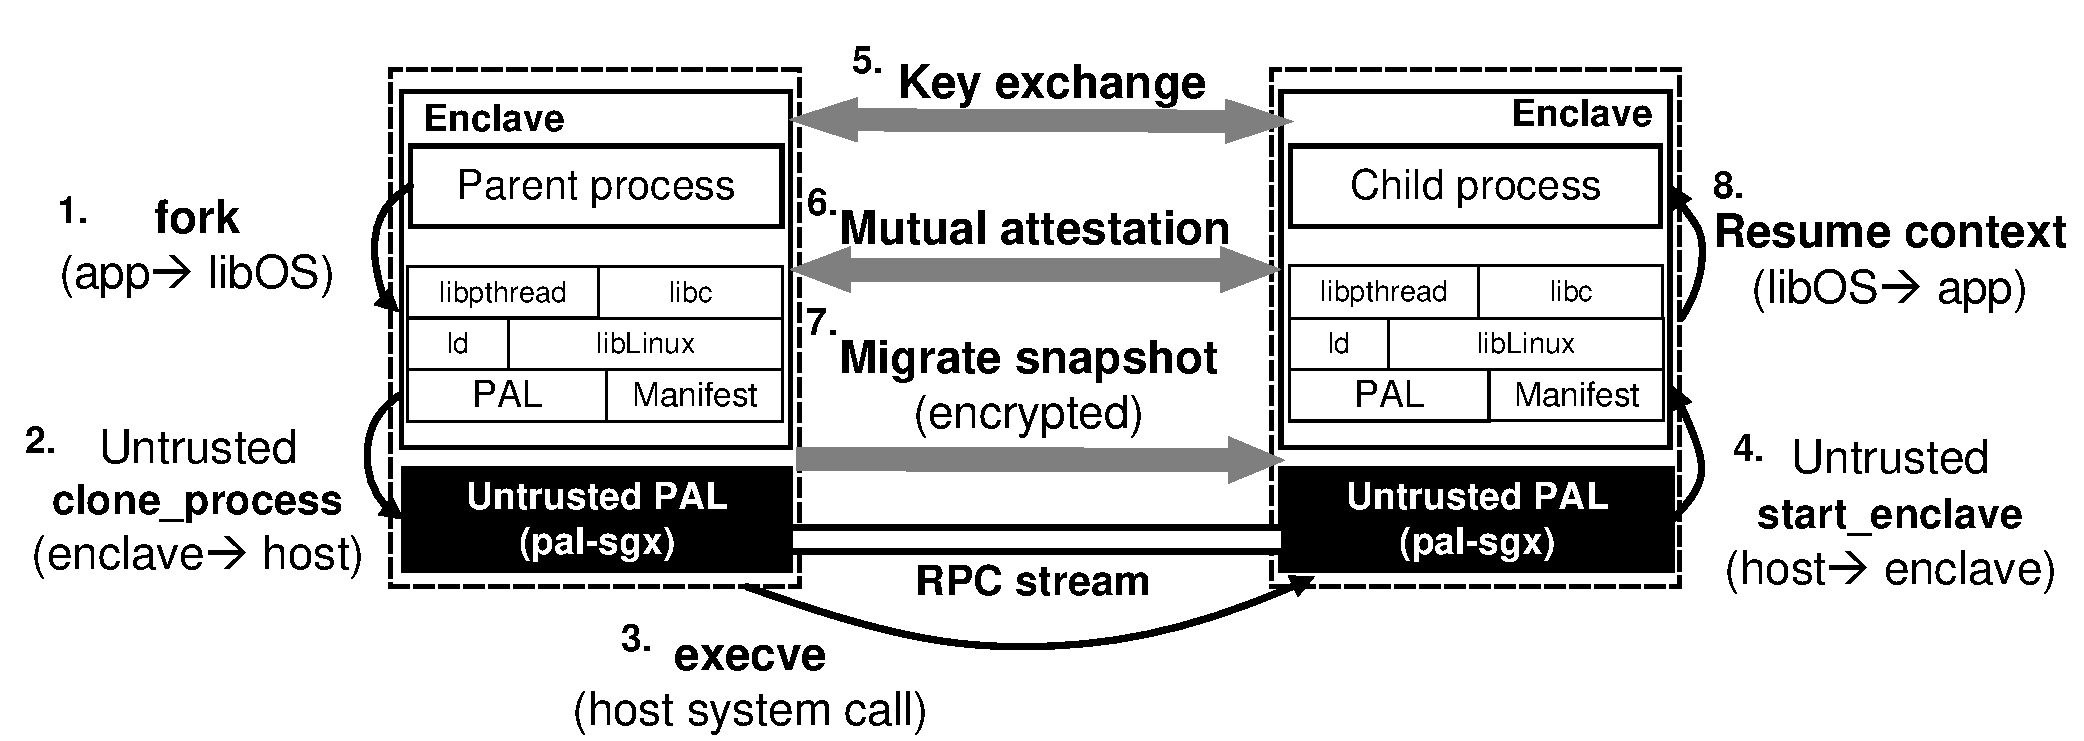
\includegraphics[width=6.5in]{graphene-sgx/figures/fork.pdf}
\footnotesize
\caption[Process creation in \graphenesgx{}]
{Process creation in \graphenesgx{}.
Numbers show the order of operations.
When a process forks, \graphenesgx{} calls {\tt execve} system call
on the untrusted host,
to create a clean enclave with the same \libos{} image.
Then the two enclaves build up the mutual trust by
exchanging a session key, verifying attestation of each other,
and migrating the process snapshot from the parent.}
\label{fig:graphene:sgx-fork}
\end{figure}

To securely create process across enclaves,
\graphenesgx{} builds trusted paths for enclaves to send process snapshots and coordinate shared states.
Since the enclaves do not directly share pages,
the coordination must be intermediated by the untrusted host.
The untrusted host may launch attacks on the multi-process abstractions of \graphenesgx{},
by either counterfeiting the behavior of either the forking or forked process,
or acting as man-in-the-middle between two processes.

%is capable of building up the trust to newly launched enclaves,
%through cooperation with an untrusted host.
%Once a clean and trusted new enclave is launched,
%The parent process will send a snapshot to the new one,
%to create a clone of itself.
%Snapshotting and migrating process states
%is a feature robustly implemented and heavily used in \graphene{} \libos{},
%of which we simply inherit the design.

When a isolated process forks,
\graphenesgx{} requests the untrusted host to create a clean enclave
of the forking process.
The parent and child process in their own enclaves
will coordinate over an encrypted RPC streams,
with the session key exchange at the beginning of coordination.
After securing the RPC streams,
the participating processes exchange attestation,
ensuring both sides are restricted to running the same application.
Once the mutual trust is built between the two processes,
further inter-process coordination is secured.
%because the parent and the child will be running the same binary,
%both enclaves can simply be expected to have the same measurement.
%To build up the trust, the two processes will open an encrypted channel
%using a session key,
%and exchange attestation generated by the processor.
%Once both sides have confirmed the integrity of the other,
%the parent process is safe to send its snapshot, encrypted, to the child
%through the said channel.
%The child process will restore the snapshot in its own enclave,
%making it a clone of its parent.
The design of process creation in \graphenesgx{} is shown as Figure~\ref{fig:graphene:sgx-fork}.

%Forking in \graphenesgx{} mainly defends against 3 types of attacks
%from the untrusted host:
%
%\begin{compactenum}
%
%\item The host pretends to be the child enclave, to expose the process snapshot
%sent from the parent.
%
%\item The host pretends to be the parent enclave, to compromise the
%child process using a malicious process snapshot.
%
%\item The untrusted host becomes a man-in-the-middle, which bounces
%encrypted messages between the child and parent enclaves, with session keys
%negotiated with both sides.
%
%\end{compactenum}
%
%As described earlier, attacks 1 and 2 are prevented by mutual attestation
%between the parent and the child,
%and encrypting the channel for sending the snapshot.
%The attestation signed by the processor proves that both entities communicating
%are valid \graphenesgx{} enclaves,
%and encrypting the channel prevents the snapshot being eavesdropped or
%counterfeited by the host.

To defend against the man-in-the-middle attack, we take advantage of
a user-customized 512-bit field
in the attestation structure generated and signed by the \sgx{} hardware.
This field is filled with a SHA-256 hash value of the agreed session key,
and the current enclave ID,
to prove that the attested party is the one who agrees on the key.

%Once a parent enclave forks a child, by default the child must be trusted
%to maintain its own security,
%because the migrated snapshot discloses all information in the parent.
%Unless the binary run in the parent enclave ensures
%that no secrets is stored in the enclave memory at the time of snapshotting,
%the parent enclave cannot simply drop the trust against the child.
%For example, a pre-forked Apache web server may want to keep each worker
%that responds to HTTP requests isolated,
%to avoid being compromised by one attacked worker.
%\graphene{} \libos{} provides an API for applications like Apache to explicitly
%specify isolation to untrusted child processes.
%\graphenesgx{} inherits the ability of dynamic process isolation,
%but developers are responsible for keeping confidential information
%from the untrusted children.

\paragraph{Implementing {\tt execve}.}
Unlike {\tt fork}, {\tt execve}
starts a process with a specified binary, often different from the callers,
in a clean process state.
%When a thread in the process, either single-threaded or multi-threaded,
%calls {\tt execve} in \graphenesgx{},
%\libos{} will migrate the calling thread to a new process,
%with clean process states except opened files cloned from the parent.
A key challenge for implementing {\tt execve} is to
identify trusted binaries that can be loaded into new enclaves as child processes.
Although a child process created by {\tt execve} does not start with
a snapshot of its parent,
The processes share states through inheriting file handles,
or future inter-process coordination.
The communication between the processes must be considered internal interaction of the application,
thus shall be protected from the host.

%Consider the case where the parent process and its child shares
%a multi-process abstraction (e.g., message queue).
%Even if only the parent side is provisioned by the client, the child side
%can still potentially compromise the secrets,
%by exploiting vulnerabilities in the shared abstraction.
%The trust between the parent and the child must be mutual,
%unless the two enclaves are strictly isolated.

As securing {\tt fork}, {\tt execve} is secured by the attestation of
the child processes' measurements.
\graphenesgx{} only allows a isolated process to create a child process
in an enclave whose measurement is listed in its manifest.
In addition, a child process does not verify the measurement of its parent,
but instead presents the measurements of all ancestors
to remote trusted server when attesting its own integrity.
In other word, for the same binary {\tt ls} isolated in the enclave,
the measurement reflects the distinction if the binary is called by,
say a shell or Apache server.

%To identify binaries that can be trusted (either as parents or children)
%during process creation,
%\graphenesgx{} requires each binary ported for an application,
%to be shipped with a list of binaries that can be {\tt execve}'d,
%and those that can be callers of {\tt execve} to the said binary.
%Each binary in the list is identified by its measurement, which is mutually attested
%between the parent and the child during process creation.
%This list must be signed by a private key provided by the client,
%while the public key must be included in the enclave measurement of the binary.

%\subsection{Securing Inter-Process Coordination}
%\label{sec:graphene:multiproc:ipc}
%
%After process creation, multiple processes in an application amy cooperate
%through sharing multi-process abstractions,
%such as signals or message queues.
%In \graphene{}, \picoprocs{} coordinate over RPC streams,
%to maintain the state of shared objects,
%as well as 
%the namespace states such as in which \picoprocs{} these objects are proxied.
%
%\graphene{} coordinates multi-process abstractions and namespaces
%by passing messages over RPC streams.
%Such a design is beneficial for supporting multi-process abstractions in enclaves.
%\graphenesgx{} inherits the same design of inter-process coordination,
%and the RPC streams used for coordination can be secured by the enclaves proactively on untrusted hosts.

%In \graphene{}, security isolation among multi-process abstractions,
%regardless of their semantics,
%are enforced by isolating the RPC streams used for coordination.
%Unfortunately, \graphenesgx{} cannot trust the host to faithfully isolate
%the RPC streams.
%Each enclave launched for an application must secure inter-process coordination
%spontaneously, by only communicating to enclaves that it has attested
%and exchanged secret keys with.
%Because inter-process coordination is completely transparent
%to the applications,
%all information sent over RPC streams must be encrypted,
%because \libos{} cannot determine whether the information may contain any secret.


